\documentclass[11pt,letterpaper]{article}
\usepackage[T1]{fontenc}
\usepackage{lmodern}
\usepackage[margin=0.92in,top=0.88in,bottom=0.9in,headheight=15pt]{geometry}
\usepackage{amsmath,amssymb,amsthm,booktabs,graphicx,tabularx,longtable,array,enumitem,xcolor,hyperref,xurl,fancyhdr,microtype}
\definecolor{ink}{HTML}{132F40}
\definecolor{accent}{HTML}{146967}
\hypersetup{colorlinks=true,linkcolor=accent,urlcolor=accent,citecolor=accent,pdftitle={Finite queries in constructive analysis},pdfauthor={OpenAI}}
\pagestyle{fancy}\fancyhf{}\lhead{\small\textsc{Constructive analysis in iPRA}}\rhead{\small\textsc{Finite queries}}\cfoot{\thepage}
\newtheorem{theorem}{Theorem}[section]
\newtheorem{lemma}[theorem]{Lemma}
\newtheorem{proposition}[theorem]{Proposition}
\newtheorem{corollary}[theorem]{Corollary}
\theoremstyle{definition}\newtheorem{definition}[theorem]{Definition}
\newcommand{\Q}{\mathbb{Q}}\newcommand{\N}{\mathbb{N}}\newcommand{\R}{\mathbb{R}}
\newcommand{\eps}{\varepsilon}
\newcommand{\ipra}{\mathrm{iPRA}}
\newcommand{\repo}[2]{\href{https://github.com/VladimirReshetnikov/ProveIt/blob/b2341af5370cd8a43f72ebb2341c0d7d7395b634/Logic/PrimitiveRecursiveArithmetic/#1}{#2}}
\newcommand{\rdir}[2]{\href{https://github.com/VladimirReshetnikov/ProveIt/tree/b2341af5370cd8a43f72ebb2341c0d7d7395b634/Logic/PrimitiveRecursiveArithmetic/#1}{#2}}
\setlist{itemsep=3pt,topsep=5pt}
\setcounter{tocdepth}{1}
\setlength{\emergencystretch}{2em}
\raggedbottom
\begin{document}
\thispagestyle{plain}
{\color{accent}\sffamily\small RESEARCH REPORT \hfill 20 NOVEMBER 2026}\par
\vspace{8pt}{\color{ink}\Huge\bfseries Finite queries in constructive analysis}\par
\vspace{5pt}{\Large Primitive-recursive moduli, integration and root finding}\par
\vspace{13pt}
\noindent A computation on a real number may ask for its ten-thousandth digit without using the preceding digits. A precision bound that records only the largest address loses this distinction. We retain the actual finite assignments that lead to each answer. They suffice to calculate the least prefix needed by a finite observation, test agreement at the two binary expansions of a dyadic point, and integrate by weighting the leaves. The proofs use finite arithmetic and give explicit primitive-recursive (PR) constructions.\par
\medskip
\noindent Two applications use different kinds of finite information. A finite difference forces a usable sign in every bracket of a monic real polynomial, even for named coefficients and repeated roots. A bounded-difference code gives finite nets of genuine Lipschitz functions on a cube, with the correct order of metric entropy. Each construction states the information its input must supply.\par
\medskip
\noindent\textbf{Formal status.} The archive contains a kernel-checked generator of object-iPRA proofs for replay of fixed binary decision trees. The general analytic results have human proofs, supporting Lean lemmas and an object-language implementation plan. The full analytic endpoint sequents are open formalization tasks.\par
\medskip\hrule\smallskip
\tableofcontents
\clearpage
\section{From finite oracle runs to arithmetic proofs}
\label{sec:framework}
\subsection{The language and its analytic interpretation}
The ordinary iPRA of ProveIt uses intuitionistic first-order logic with equality, a numerical sort, defining equations for each PR symbol, the successor axioms, and induction for quantifier-free formulas. For instance, the assertion that a rational sequence is regular is a formula about numbers. With $\eps_i=2^{-i}$ it is
\[
   \forall i,j\quad |a(i)-a(j)|\le\eps_i+\eps_j .
\]
For a fixed PR term $a(e,i)$, $e$ may be an object variable. Rationals can be encoded as a signed integer and a positive denominator. Order and the displayed inequality are PR Boolean tests by clearing positive denominators. Two regular names are equivalent when $|a(i)-b(j)|\le\eps_i+\eps_j$ for every $i,j$. In the metric completion these clauses say that the names converge with the displayed errors and represent the same point. All input names for $[0,1]$ can be clamped to this interval. Clamping is rational and 1-Lipschitz.

In the sequel, quantification over machines, coefficient routines or names without a numerical code is at the metalevel. A theorem about such a family means that fixing its PR definitions yields a numerical sequent from its stated arithmetic contracts. Contract assumptions can have number quantifiers. Induction inside the sequent is always on a numerical loop with a quantifier-free, or Boolean-compiled bounded, invariant. Here iPRA has neither function variables nor a total PR evaluator for every PR program. Arbitrary Type-2 oracles appear in semantic adequacy proofs. For object use we substitute a fixed term for a query or supply a finite coded table.

\subsection{The existing interfaces and the change made here}
\begin{center}\small
\begin{tabularx}{\linewidth}{@{}>{\raggedright\arraybackslash}p{.29\linewidth}X@{}}
\toprule
Repository component & What is reused or strengthened\\ \midrule
\repo{README.md}{Ordinary iPRA} and \repo{Derivations/README.md}{its derivation library}
& The target judgment is an actual derivation $\Gamma\vdash_{\rm PRAAx}\varphi$. Finite executable checks and mathematical interpretations have separate roles.\\[3pt]
\repo{docs/proofs/foundations/ipra_finite_query_normal_form_2026-11-16/metadata/DIFFICULTY_MATRIX.csv}{Finite-query difficulty matrix} (D4, D12, D17)
& It identifies a missing PR modulus or compactness witness as a producer obligation. We construct a modulus from clocked, finitely branching access to the input, including the compatibility test needed on the interval.\\[3pt]
\repo{docs/proofs/analysis/calculus_ipra/README.md}{Constructive calculus} and \repo{Derivations/Lean/IPRADerivations/Foundations/FiniteUseSignObstruction.lean}{finite-use sign obstruction}
& The calculus packet takes continuity data as input. The sign metatheorem already proves replay for a fuelled machine. Here we use replay to recover exact finite oscillations and dyadic masses.\\[3pt]
\repo{docs/proofs/foundations/ipra_continuous_framework_2026-11-20_2/paper/sections/07_limits.tex}{Continuous-structures limits} and \repo{Derivations/Lean/IPRADerivations/Analysis/PolynomialRootName.lean}{polynomial root names}
& The former supplies Lipschitz envelopes and recovery from small residual diameter. The latter handles rational polynomial data by exact signs. Sections \ref{sec:root-realizer} and \ref{sec:entropy} give a different sign producer and a smaller function-space code.\\
\bottomrule
\end{tabularx}
\end{center}
These comparisons use the linked files at commit \texttt{b2341af5370c}. Dialogue interpretations of computation and modulus extraction from represented programs have a substantial history \cite{escardo,pauly}. The contribution here is a numerical specialization with an optimal finite-prefix formula, a sparse test for dyadic identifications, and a shared aggregation algorithm. No priority claim is needed for those underlying techniques.

\subsection{Machines with a clock}
A request has a parameter $e$ and precision $k$. Fix PR functions for initialization, the action at a state, transition on an answer, and extraction of a rational result. Actions are halt, internal step, or ask the bit at a natural address $q$. A PR clock $B(e,k)$ bounds all steps on consistent answers. An explicit decision tree of depth at most $B$ is another presentation. Inconsistent answers to a repeated query need never be explored. To make all operations total, run with fuel $B$, inspect the state after the last step, and use a distinguished failure value on a nonterminal state. The clock contract excludes that value on reachable paths.

Start at the root with an empty finite map. Follow an internal transition with this map unchanged. At an old query follow the unique stored answer. At a new query fork with that coordinate set first to zero and then to one. A terminal row $s$ consists of the finite partial assignment $P_s$ and rational output $v_s$. We denote the resulting list for precision $k$ by $L_k$ and suppress $e$. A row describes all inputs extending $P_s$. Each extension follows exactly this run, by induction on its remaining steps. Conversely every run follows one row because the next actual bit chooses its unique successor. Distinct rows disagree on a common coordinate, namely the first query at which their runs branched. Every row is nonempty as a set of inputs, since unspecified bits may all be filled with zero.

For a single oracle, replay needs agreement only on the addresses visited. For composition, replace each outer request by an inner run that returns its answer. By induction at the outer node, the result agrees with direct evaluation on the simulated oracle. Its query list concatenates the inner query lists in outer execution order. For outer query depth $b$ and inner query depth at most $c$ on those requests, the composite uses at most $bc$ primitive reads. In a state-machine implementation whose clocks charge internal steps as well, if $b,c$ instead bound total outer and inner steps, then $b(c+2)+1$ transitions suffice with unit-cost call and return. If the inner clock depends on the request, enumerate the reachable outer requests and take their maximum before applying this bound. This last step needs a finite answer alphabet or a separate bound on answers. Typed generalizations of replay and substitution are checked in the accompanying Lean code.

\paragraph{Primitive recursion and cost.}
At most $2^B$ terminal rows and $2^{B+1}-1$ explored state occurrences suffice even with unary transitions. One particularly simple PR construction simulates the $2^B$ padded strings of possible fresh answers and removes repeated paths. Each simulation takes at most $B$ steps. This proves PR definability independently of the implementation's traversal order. An explicit stack visits the pruned tree once, stores at most $B$ coordinates per path, and avoids the redundant simulations. Taking the largest reached address supplies an upper bound for all the addresses. Cost statements about numbers of rows, queries or comparisons do not count the bit cost of a PR transition or of rational arithmetic.

\subsection{The exact prefix needed by a finite observation}
For a tolerance $\eta\in\Q_{\ge0}$, call $N$ safe at precision $k$ if streams agreeing at coordinates $q<N$ give outputs differing by at most $\eta$. For a pair of rows define $D(s,t)=\{q\in\operatorname{dom}P_s\cap\operatorname{dom}P_t:P_s(q)\ne P_t(q)\}$.
\begin{theorem}[Least safe prefix]\label{thm:least}
The least safe prefix length is
\[
   M_k(\eta)=
   \max\bigl(\{0\}\cup
   \{1+\min D(s,t):s,t\in L_k,\ |v_s-v_t|>\eta\}\bigr).
\]
\end{theorem}
\begin{proof}
A pair of rows has extensions agreeing below $N$ precisely when it has no conflicting shared requirement there. For the reverse implication, fill each low coordinate from the left map if present, otherwise from the right, otherwise by zero. Above or at $N$ fill the two maps separately. These explicit extensions are PR functions of the finite data. For rows whose values differ by more than $\eta$, $D(s,t)$ is nonempty by the first divergent branch. Agreement below $N$ excludes this pair exactly when $N>\min D(s,t)$. Taking the maximum proves sufficiency and necessity, including the case of no forbidden pair. If $N$ is too short the construction supplies two counterexample streams.
\end{proof}
The minimum is sharp for the \emph{given finite observation}. Different approximation programs for the same continuous function can have different finite optimal prefixes. For example a program that asks bit $10^6$ but ignores the reply has exact use zero when its result is constant. One can compute all pairwise conflicts using at most $O(|L_k|^2 B^2)$ address comparisons with unsorted lists. This bound has no factor equal to the largest address.

\section{An interval modulus from the program}
\label{sec:interval}
The binary chart sends bits $\alpha(0),\alpha(1),\ldots$ to $\sum_{q\ge0}\alpha(q)2^{-q-1}$. A prefix of length $N$ describes a closed interval of width $2^{-N}$. The sole overlaps at a given level are neighboring endpoints. We use precisely these overlaps to pass from a prefix modulus to a Euclidean one. No procedure for finding a binary expansion of an arbitrary constructive real is needed.

\subsection{Two finite arithmetic tests}
Write $v_k(\alpha)$ for the output of one run. For finite partial maps $P,T$ write $P\parallel T$ when they agree on common addresses. The following are universally indexed hypotheses, each individual instance a decidable finite test:
\begin{align}
 |v_s-v_t| &\le \eps_k+\eps_l
 &&(s\in L_k,\ t\in L_l,\ P_s\parallel P_t), \tag{C}\label{eq:C}\\
 |v_s-v_t| &\le 2\eps_k
 &&(s,t\in L_k,\ \operatorname{Carry}(P_s,P_t)). \tag{G}\label{eq:G}
\end{align}
Here $\operatorname{Carry}(P,T)$ means that $P$ and $T$ extend, respectively, to the lower-cell and upper-cell expansions $u0\,111\ldots$ and $u1\,000\ldots$ of an interior dyadic. The digit at address $j=|u|$ is the carry. This apparently unbounded condition has a short decision procedure.

\begin{lemma}[Sparse carry test]\label{lem:carry}
Let $A=\operatorname{dom}P\cup\operatorname{dom}T$. It suffices to test $j$ in
$\{0\}\cup A\cup\{q+1:q\in A\}$. At each candidate require:
\begin{enumerate}[label=(\roman*),leftmargin=24pt]
\item below $j$, no address is assigned different bits by both maps.
\item at $j$, any specified left bit is $0$ and any specified right bit is $1$.
\item above $j$, all specified left bits are $1$ and all specified right bits are $0$.
\end{enumerate}
\end{lemma}
\begin{proof}
These conditions are necessary. When they hold, fill the common prefix by the union of the restricted maps, putting zero in empty positions. Append the indicated differing bit and constant tails. This proves sufficiency with concrete total extensions. A candidate in $A$ is tested itself. For $j$ outside $A$, all three tests depend only on the gap of the ordered addresses containing $j$. The first integer of that gap is zero or the successor of an address. It gives exactly the same outcomes, including in the infinite last gap.
\end{proof}

Condition (C) is equivalent to regularity at all pairs of precisions on a single bit stream because compatible maps have the explicit common extension obtained by filling their union with zeros. Given (C), condition (G) is equivalent to equality of the two named values on every dyadic overlap. Indeed, equal completed values give the bound $2\eps_k$ by the two approximation errors. Conversely, comparison through a common fine level $r$ on both expansions gives the mixed bound $\eps_k+\eps_l+4\eps_r$. Any positive excess over $\eps_k+\eps_l$ would be a rational gap contradicted by a sufficiently fine $r$. This tightening uses only rational order. For a gap $a/b>0$ in lowest terms one can, for example, take $r=b+4$. The tests are obligations for all precisions. Passing finitely many tests on a program does not establish those obligations.

\subsection{The translation theorem}
For a rational $x\in[0,1)$ use its terminating-zero convention at dyadics, and at $1$ use all ones. Its bit at $q$ is $\lfloor 2^{q+1}x\rfloor\bmod 2$, except for that endpoint. Let $V_k(x)$ be the output on this particular rational name. Binary digits of rationals are PR, including for non-dyadic rationals. If $x=a/b$, one may first reduce $a2^{q+1}$ modulo $2b$ and compare to $b$. This modular powering avoids constructing a prefix of length $q$.

\begin{theorem}[Conversion in both directions]\label{thm:interval}
A clocked binary evaluator satisfying (C) and (G) induces an extensional function on regular Cauchy names in $[0,1]$, with a PR Euclidean modulus. In particular, take $N_k=M_k(0)$. A modulus for error $\eps_j$ is
\[
                    \mu(j)=N_{j+2}+1 .
\]
Conversely, a fixed PR rational evaluator with a supplied PR uniform modulus and the usual mixed-precision error contract on $[0,1]$ has a clocked binary evaluator satisfying (C) and (G) for the same function.
\end{theorem}
\begin{proof}
First consider rationals $x,y$ with $|x-y|\le 2^{-N}$, $N=M_k(\eta)$. If they lie in the same prefix cell, their observed outputs differ by at most $\eta$. Otherwise the canonical cell indices $\min(2^N-1,\lfloor 2^Nx\rfloor)$ and its analogue for $y$ differ by one. The two expansions of the common endpoint have the respective cell prefixes. Comparison with these two expansions, with (G) between them, gives
\begin{equation}
            |V_k(x)-V_k(y)|\le 2\eta+2\eps_k.             \tag{1}\label{eq:adj}
\end{equation}
This works at $0$ and $1$ as well. At $N=0$ only the single-cell case occurs. In particular the rational observation at $\eta=0$ varies by at most $2\eps_k$ over the indicated distance. By (C), $V_k(x)$ is a regular name at each rational $x$.

Here is the actual evaluator on a regular input $a$. Define
\[
 H(k)=\max_{i\le k}N_i,\qquad p(n)=H(n+3)+2,\qquad
                         y_n=V_{n+3}\bigl(a(p(n))\bigr).
\]
For $m\ge n$ the two rational arguments lie within $2\eps_{p(n)}\le 2^{-N_{n+3}}$. Apply (1) at level $n+3$ followed by (C) at the second argument. This gives
\[
                |y_n-y_m|\le3\eps_{n+3}+\eps_{m+3}
                         \le\eps_n+\eps_m .
\]
The same proof with two equivalent input names gives the mixed inequality $|y_n(a)-y_m(b)|\le\eps_n+\eps_m$ (interchange them when $n>m$). Thus the evaluator respects name equality. Constant input names give the original rational values.

For the Euclidean modulus, fix $k=j+2$ and suppose two represented inputs are at distance at most $2^{-N_k-1}$. In finite comparisons their samples of sufficiently high precision differ by at most $2^{-N_k}$ because the spare half-cell pays for both sampling errors. On these rationals (1) with $\eta=0$ bounds the difference at level $k$ by $2\eps_k$. Comparing each fine observation at level $n+3$ with its level-$k$ observation by (C) costs at most $2(\eps_k+\eps_{n+3})$ in total. Letting the rational slack decrease gives the bound $4\eps_k=\eps_j$. More explicitly, for arbitrarily fine sample indices use $p(n)\ge H(k)+2$ when $n+3\ge k$, so both input sampling errors are at most $2^{-N_k-2}$. The terms $2\eps_{n+3}$ and the output regularity errors tend to zero. If $p(n)$ stays bounded, that same half-cell estimate still applies. All comparisons can be made with the finite definition of distance $\le r$, namely $|a_i-b_l|\le r+\eps_i+\eps_l$.

A bit stream itself presents a regular name by truncation to $n$ digits (tail $\le\eps_n$). Its image under the new evaluator equals its old output name. For a fixed $k$ compare to the rational truncation of length $p(n)$. Whenever $n+3\ge k$ it shares the first $N_k$ bits. Even when the infinite stream ends in all ones, each finite truncation is strictly below 1 and its terminating expansion has the prescribed finite prefix. Hence its level-$k$ observation agrees exactly with the original for these truncations. Use (C) on the truncation and then let the precision grow. This also explains why ordinary nonredundant binary digits cause no discontinuous choice in the translation.

Conversely let $E(x,p)$ approximate the value at rational $x$ with error $\eps_p$, with modulus $\nu$ on completed values. At output level $k$, read $m=\nu(k+1)$ initial bits and use $E(u/2^m,k+1)$, where $u$ is their unsigned integer. The stream's point is within $2^{-m}$ of the truncation. The modulus and sample error give at most $2\eps_{k+1}=\eps_k$ total error. This implies (C) and (G). Directly in finite arithmetic, compare any two truncations of one stream through a longer common truncation. Each is within the mesh of its own requested modulus. Applying the mixed evaluator inequalities through a fine intermediate evaluation gives (C) after the rational slack is removed. At a carry use the common rational endpoint instead. This proves the same bounds without quantifying over real points. The finite prefix loop and the fixed evaluator have PR state descriptions and clocks in the stated PR operation model.
\end{proof}

For immediate use by a rational-domain client, set $E(x,p)=V_p(x)$. On qualifying rational pairs compare $V_p(x)$ and $V_q(y)$ through level $j+2$ at both arguments. Equations (C) and (1) give exactly $\eps_p+\eps_j+\eps_q$. Thus the hypotheses used by the root and calculus routines are available with an explicit $\mu$. The bounds also extend coordinatewise to a fixed product of intervals by tagging queries by coordinate, applying the carry condition with common other coordinates and changing one coordinate at a time. For $d$ factors the sum of the $d$ coordinate errors replaces the single error. Requesting $\lceil\log_2 d\rceil$ extra bits per coordinate suffices.
\paragraph{Discarding digits that change only the rounding error.}
Equation (1) also offers a cheaper modulus when exact finite equality is too demanding. With $k=j+3$ and $\eta=\eps_k$, completed inputs at distance at most $2^{-M_k(\eps_k)-1}$ give output distance at most $2\eta+4\eps_k=6\eps_k\le\eps_j$. To see this without assuming that the original Cauchy-name evaluator samples sufficiently finely, represent each input by its shifted name $a'(i)=a(i+M_k(\eps_k)+3)$, and use the proved extensionality. Equivalently, the original samples already suffice because $M_k(\eps_k)\le N_k$ and eventually $p(n)\ge N_k+2$. Take the smaller of this modulus and the exact-prefix modulus from Theorem~\ref{thm:interval}. As an example, the program returning $\eps_{k+2}\alpha(J)$ represents the zero function. Its least exact prefix has length $J+1$, while its least prefix at tolerance $\eps_k$ is zero. The optimization concerns input precision. The finite output is still obtained from its specified program.

\section{Integration and extrema without a full grid}
\label{sec:aggregation}
Write $d_s=|\operatorname{dom}P_s|$. There are two different costs of reading a far-away digit. Computing an individual digit at a rational argument may require arithmetic on its address. Enumerating all assignments to every earlier digit can be avoided altogether.

\begin{theorem}[Three constructive observations]\label{thm:agg}
Under (C) and (G) the following rational outputs have error at most $\eps_k$ for the minimum value, the ordinary Riemann integral on $[0,1]$, and the maximum value of the represented function:
\[
       \min_{s\in L_k}v_s,\qquad
       I_k=\sum_{s\in L_k}2^{-d_s}v_s,\qquad
       \max_{s\in L_k}v_s .
\]
All three outputs satisfy the mixed regular-name inequality across levels. A row with maximal value yields a rational point within $2\eps_k$ of the supremum in value. The minimum has the same conclusion.
\end{theorem}
\begin{proof}
Choose $U$ one greater than the greatest address used at level $k$, taking $U=0$ when there are no queries. Among the $2^U$ words of length $U$, exactly $2^{U-d_s}$ extend a prescribed row. Fill each unused address independently to see this bijection, which counts the empty word once at $U=0$. The row families partition the words. Consequently their weights sum to one and $I_k$ is the exact mean of the full table. Repeated reads impose the same constraint and count only once. Any common denominator for the leaf values needs at most another factor $2^{\max_s d_s}$ for this mean, irrespective of $U$.

Given levels $k,l$, use words at their common largest width. For each word the two visited rows are compatible, and (C) bounds their output difference by $\eps_k+\eps_l$. Averaging proves regularity of $I$. Every row at either level has an extension, so the same comparison proves the two extremal inequalities in both directions. This is already an arithmetic derivation of the name contracts. No completed integral or extremum was assumed.

For the integral interpretation, divide $[0,1]$ into the dyadic cells of width $2^{-U}$. At every rational point in a cell interior, the level-$k$ canonical observation is its table entry. The limiting rational-domain value differs from that entry by at most $\eps_k$ by (C). By the proved uniform continuity, this bound extends to the closed cell, including the endpoints (approach from the interior with rational points). Quantitatively, an endpoint can equivalently use that cell's own endpoint expansion, and positive gaps are eliminated by the rational slack argument used for (G). On a dyadic refinement of these cells, each Riemann tag value therefore differs from its parent entry by at most $\eps_k$. The sum of subinterval lengths is one. The tagged sum is within $\eps_k$ of $I_k$. For arbitrary sufficiently fine tagged partitions, refine by their union with the dyadic partition. Compare tags within the original subintervals using the modulus from Theorem~\ref{thm:interval}. Mesh at most $2^{-\mu(j)}$ adds at most $\eps_j$ in total. Thus arbitrary fine rational Riemann sums converge to the name $I$. This proves adequacy with an explicit error estimate and avoids a measure-existence axiom.

For the upper extremum, all rational-domain values are bounded by $\max v_s+\eps_k$, and the bound extends to completed inputs by continuity. Take a maximizing row and set unassigned bits equal to zero. The resulting finite-support expansion gives a rational point with value at least $\max v_s-\eps_k$. The supremum is the named least upper bound. Indeed, all values satisfy the preceding upper estimate, and any proposed upper bound must bound the explicit near-witness at each precision. A rational gap to the name is contradicted by choosing $2\eps_k$ smaller than that gap. Negate outputs to obtain the lower extremum. The near-witnesses need not converge to one maximizing point.
\end{proof}

\begin{figure}[htbp]
\centering
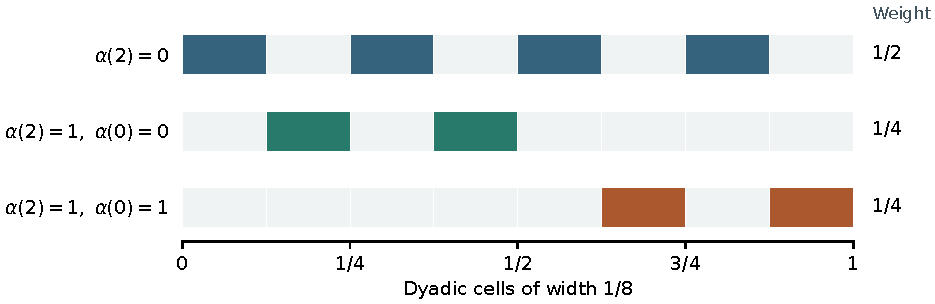
\includegraphics[width=.85\linewidth]{figures/sparse-cylinders.pdf}
\caption{A program first asks for bit 2, and asks for bit 0 only when the reply is one. Color shows the cells reaching each terminal row. The unqueried bit 1 has already been summed out. Row weights require only the number of distinct answers on that path.}
\end{figure}

The averaging proof works on Cantor space already from (C). Condition (G) is what allows us here to speak of an extensional \emph{continuous} function of a Cauchy real. The integral of the first binary digit as a step function also exists, although that digit fails (G). This illustrates the distinction between the finite counting identity and the analytic interface chosen in Theorem~\ref{thm:interval}.

\subsection{A high-frequency calculation}
Let $T(t)=2\min(\{t\},1-\{t\})$, with the periodic extension at integers. For $J\ge0$ consider $f_J(x)=T(2^J x)$. At precision $m\ge1$, read just the $m$ bits with addresses $J,\ldots,J+m-1$. Treat them as the integer $v<2^m$ and return
\[
                   T\big((v+1/2)2^{-m}\big).
\]
On either expansion of any point the fractional phase belongs to the closure of the corresponding phase bin, with $0$ and $1$ identified. Since $T$ is 2-Lipschitz on each period and matches across the boundary, the error is at most $\eps_m$. For level zero use the constant $1/2$. Thus (C) and (G) hold. Each half-period is linear, so the midpoint rule is exact on every bin for $m\ge1$ and the mean is exactly $1/2$. Alternatively, sum the symmetric arithmetic progression of the $2^m$ leaf values. Sparse integration does this computation without representing the $2^J$ periods.
\begin{center}
\begin{tabular}{rrrrr}\toprule
$J$ & sampled digits $m$ & leaves & least exact prefix & mean\\\midrule
0 & 6 & 64 & 6 & $1/2$\\
5 & 6 & 64 & 11 & $1/2$\\
10,000 & 6 & 64 & 10,006 & $1/2$\\\bottomrule
\end{tabular}
\end{center}
For $m=6$, changing the last inspected digit of the first bin changes its midpoint value. The least exact prefix is therefore $J+6$, even though each path reads six bits. A literal prefix table in the last row would have $2^{10006}$ entries. The comparison is with that particular table representation. A specialized formula for the tent's integral also immediately gives $1/2$. The sparse tree works without recognizing that formula.

\subsection{Gluing intervals on a finite metric graph}
Let a finite connected graph have at least one edge, no isolated vertices, and positive rational edge lengths $\lambda_e$. Loop edges and parallel edges are allowed. Give each oriented edge its own unit-interval bit evaluator satisfying (C) and (G). For every two incidences at a vertex require that the two corresponding constant endpoint streams at level $k$ have outputs differing by at most $2\eps_k$, for every $k$. This includes the two ends of a loop. It is a finite scan at fixed $k$. Comparing at an arbitrarily fine intermediate level using (C) proves the mixed endpoint inequalities, hence the edge limits give a common vertex value.

\begin{corollary}[Gluing and averaging on a graph]
These data yield a PR evaluator on regular names for the path metric of the graph, a PR modulus on the whole graph, and a regular name for its normalized arclength integral:
\[
             \frac{\sum_e\lambda_e I_{e,k}}{\sum_e\lambda_e}.
\]
\end{corollary}
\begin{proof}
Take rational edge positions as the dense codes. Distances are rational and PR in the coded finite graph. On one edge include the direct path. Also try each choice of an endpoint of each of the two incident edges, add the initial and terminal partial lengths, and minimize the intervening vertex-to-vertex distance. For the latter enumerate simple vertex paths with their edge choices up to the vertex bound, since removing any cycle shortens a path. The empty path is admitted between identical vertices. This computation proves that a minimum is attained on the finite dense problem.

Let $\mu_e(j+1)$ be the interval modulus already computed at target $j+1$. Choose a dyadic $r=2^{-m}$ with
\[
  0<r\le \tfrac12\min_e\bigl(\lambda_e\,2^{-\mu_e(j+1)}\bigr).
\]
To make this choice by a PR calculation, observe that if the right side is $a/b>0$ for positive integers, $m=b$ works, and bounded minimization up to $b$ gives a smaller exponent if desired. In particular $r$ is strictly shorter than any whole edge. A shortest path of length at most $r$ is therefore direct along an edge, or consists of two partial edges meeting at a single vertex. For either partial segment its normalized length is within the modulus of its edge, so its change in limiting value is at most $\eps_{j+1}$. Equality of the vertex value joins these bounds and gives $\eps_j$ in all cases. At a rational dense point evaluate its chosen edge. The endpoint tests make different incident edge codes equivalent as names. Thus the dense evaluator has a mixed bound with this explicit graph modulus. The Cauchy lift uses the same envelope-and-extra-bits argument as on the interval, now applied to the rational graph distance. In particular one need never choose an edge containing the limit of a Cauchy name. Each normalized edge integral has error $\eps_k$. Taking their convex combination preserves this error and gives the displayed arclength formula by additivity on edges.
\end{proof}
A single loop gives a periodic real domain. The endpoint test detects a simple failure. The identity function on the parameter interval passes the interior carry tests, but its values at the endpoints differ by one and cannot define a continuous function on the loop. For a triangle with edge lengths $1,2,3$ and linearly interpolated cyclic vertex values $0,1,-1$, the three edge means are $1/2,0,-1/2$. The normalized graph integral is therefore $-1/6$. The reference program verifies the three endpoint comparisons at seven precisions.

\subsection{Two limits on automatic modulus extraction}
\paragraph{An evaluation oracle without a clocked program.}
A modulus at tolerance $1/2$ cannot be computed uniformly from pointwise rational evaluations of an otherwise unrestricted continuous function. Run a proposed oracle algorithm on the zero function. It asks for finitely many rational arguments, and returns some $m$. Choose a rational subinterval avoiding all those arguments and shorter than $2^{-m}$. A rational piecewise linear tent supported there with height one agrees on every query but violates the returned modulus. The alternative construction and both evaluators are PR once the finite data are fixed. Hence the clock and transition access used for exploring all possible answers genuinely supply information. A clock for each individual black-box evaluation alone does not expose its branches in the input point.

\paragraph{A computable interval function with no PR modulus.}
Enumerate the unary PR programs effectively, with programs $p_i$. In ordinary computability theory the function $A(n)=1+\max_{i\le n}p_i(n)$ is total computable by interpreting finitely many structurally recursive programs and waiting for their evaluations. It eventually strictly exceeds every unary PR function. Consider
\[
                     g(x)=\sum_{n=1}^\infty 4^{-n}T(2^{A(n)}x).
\]
Its tail after $n$ is bounded by $4^{-n}/3$, and each finite term is computable on Cauchy reals. Computing sufficiently many terms with total error split among them gives a Type-2 computable continuous function in the external interpretation. Yet $g(0)=0$ and at $x_n=2^{-A(n)-1}$ the $n$th summand is $4^{-n}$ while every summand is nonnegative. A modulus at tolerance $2^{-(2n+1)}$ must therefore satisfy $\mu(2n+1)>A(n)+1$. A PR $\mu$ would contradict diagonal domination. The example identifies a specific limitation of embedding Type-2 computable analysis into clocked PR arithmetic even on a compact interval.

\section{Finding a real zero from finitely many noisy samples}
\label{sec:root-realizer}

A rational polynomial permits an exact sign test at each rational midpoint.
The repository's \texttt{Analysis.PolynomialBisection} uses this fact,
and \texttt{PolynomialRootName} constructs a regular root name from the
nested brackets. Its \texttt{PolynomialRootUniqueness} uses a positive
divided-difference bound to compare independently obtained names.
For a polynomial with \emph{named real coefficients} the midpoint value
may itself be an undecidable zero. We give a bounded replacement for
this sign test. It works at repeated roots and in intervals containing
several roots.

\subsection{What a modulus alone buys}

Put $e_k=2^{-k}$. A rational evaluator $E(x,p)$ on $[0,1]$ has error
$e_p$ for the continuous function $f$ it presents. Its continuity modulus
$\mu$ guarantees $|f(x)-f(y)|\le e_j$ whenever $|x-y|\le e_{\mu(j)}$.
These semantic inequalities abbreviate the rational bounds
$|E(x,p)-E(y,q)|\le e_p+e_j+e_q$ on qualifying pairs, together with
$|E(x,p)-E(x,q)|\le e_p+e_q$. A weak initial bracket means
$E(0,p)\le e_p$ and $E(1,p)\ge-e_p$ for all $p$. Evaluators and moduli
are fixed PR programs, possibly with number parameters.

\paragraph{Approximate intermediate values.}
At demand $k$, set $p=k+2$ and start with $[a,b]=[0,1]$. For at most
$\mu(k+1)$ steps sample $v=E((a+b)/2,p)$. If $|v|\le e_p$, return
the midpoint. If $v>e_p$, replace $b$ by the midpoint. Otherwise
$v<-e_p$, so replace $a$. At exhaustion return the remaining midpoint.
An early answer has residual at most $2e_p$. Each update preserves
$f(a)\le0\le f(b)$. At exhaustion the bracket has width at most
$e_{\mu(k+1)}$, so its midpoint value is both at most $e_{k+1}$ above
the left endpoint value and at most $e_{k+1}$ below the right endpoint
value. The residual is therefore at most $e_{k+1}$ in both cases.
Internally the output $z$ satisfies
$|E(z,q)|\le e_q+e_{k+1}$ for every $q$. To obtain this bound fix $q$ before induction,
using the endpoint bounds at an arbitrary auxiliary precision $t$.
For example an exhausted bracket gives
$E(z,q)\le e_q+e_{k+1}+2e_t$ for every $t$. If the claimed rational
upper bound failed, its positive rational excess would give a bounded
choice of $t$ with $2e_t$ smaller than that excess (the denominator
plus two suffices for a reduced positive rational). The lower bound
follows the same way. There are at most
$\mu(k+1)$ evaluator calls, compared with $2^{\mu(k+1)}+1$ points in
the full uniform mesh. This is a query count. The cost of a call depends
on its provider. Frank's constructive approximate IVT gives an existence
result even under pointwise continuity. Here the supplied modulus serves
to calculate the finite stopping budget.\footnote{M. Frank,
\emph{Interpolating Between Choices for the Approximate Intermediate
Value Theorem}, \href{https://arxiv.org/abs/1701.02227}{arXiv:1701.02227}.}

\paragraph{A finite-use obstruction.}
No uniform oracle algorithm can, from these same data, return a regular
name of an exact zero for every input. Consider
\[
 g(x)=\min(x-1/3,0)+\max(x-2/3,0).
\]
This function and all vertical translates are $1$-Lipschitz. Run a
hypothetical algorithm on the exact rational evaluator for $g$ to obtain
a root approximation of error at most $1/16$. Let $b$ bound the
precisions of its finitely many requests. Choose a positive dyadic
$c<\min(1/12,e_b)$. Give the two inputs $g+c$ and $g-c$ evaluators
that return $g(x)$ at precisions up to $b$ and exact values thereafter.
They have the same Lipschitz modulus and each has the required strict
endpoint crossing. The two runs have the same transcript by deterministic
replay. Their unique roots are $1/3-c$ and $2/3+c$. They are more than
$1/3$ apart, so no common answer works. This is a representation-level
impossibility even for PR families fed through their evaluators. The
argument does not concern algorithms given extra symbolic syntax. It is
the root analogue of the repository's
\texttt{Foundations.FiniteUseSignObstruction}.

\subsection{A local certificate for coherent brackets}

At stage $n$, a certificate on $I=[a,b]$ consists of a rational
$z\in[a+(b-a)/3,b-(b-a)/3]$ and a precision $p$ with
$|E(z,p)|>e_p$. A fixed PR producer of these data suffices. Retain
$[a,z]$ for a positive value and $[z,b]$ for a negative value.
Each interval is nested, retains the weak bracket, and has length
between one third and two thirds of its predecessor. Let $x_k$ be
the midpoint after $2k$ stages. Since $(2/3)^2<1/2$,
\[
    |I_{2k}|\le e_k,\qquad
    |x_l-x_k|\le e_k/2\quad(l\ge k).
\]
All runs use the same stage-indexed producer and tie rule, so they agree
on their shared prefix. This defines a regular name. Given output
residual demand $j$, use any $k\ge\mu(j)$ in the endpoint estimate
above to obtain $|f(x_k)|\le e_j$. Continuity yields $f(x)=0$ for
the named limit $x$. This proves a root relation. Different presentations
of a polynomial with several roots may produce different valid roots.
For a unique root all such outputs agree. No compatibility between
independently chosen approximate zeros is assumed.

\subsection{Producing the certificate for a monic polynomial}

\paragraph{Polynomial crossing theorem.}
Let $d\ge1$ and
$P(t)=t^d+\sum_{i<d}c_it^i$, where $c_i$ has a rational name $C(i,s)$
of error $e_s$. Suppose $P(0)\le0\le P(1)$. Then one uniform
PR algorithm in the degree and numerical parameters of the fixed
coefficient provider returns a regular name of a real zero in $[0,1]$.
It uses $2kd$ coefficient queries for position demand $k$, including
in the presence of multiple roots. For a model charging one query per
coefficient table, the count is $2k$.

\paragraph{A rational observation that forces a sign.}
For a rational monic $Q$ of degree $d$, step $h>0$, and starting point
$u$, the $d$th forward difference of $Q$ is the constant $d!h^d$.
Indeed $Q(t+h)-Q(t)$ has degree $d-1$ and leading coefficient $dh$,
by the binomial identity. Repetition gives the claimed constant.
If $M=\max_{0\le i\le d}|Q(u+ih)|$, one difference row has entries
bounded by $2M$ by the triangle inequality. Repeating gives
\[
  d!h^d\ \le\ 2^d M.                                      \tag{R1}
\]
A bounded rational scan therefore finds a large value, even when
particular probes evaluate to zero. The forward differences are used
in the proof only.

\paragraph{Precision and cost.}
Let $w=b-a$ at stage $n$, set $u=a+w/3$, $h=w/(3d)$, and use
the $d+1$ points $u+ih$ in the middle third. Write
$\ell(v)=\min\{r\le v:2^r\ge v\}$ for positive integer $v$.
Use
\[
   p_n=d\bigl(\ell(6d)+2n\bigr)+3,\qquad s_n=p_n+\ell(d).
\]
Read each of the $d$ coefficients once at $s_n$ and form the monic
rational polynomial $Q_n$ with those coefficients. On $[0,1]$,
$|P-Q_n|\le d e_{s_n}\le e_{p_n}$. Because $w\ge3^{-n}$,
\[
   \frac{d!h^d}{2^d}\ \ge\ (6d\,3^n)^{-d}\ \ge\ 8e_{p_n}.
\]
Choose the least node index attaining the maximum in (R1). Its
$Q_n$-value has magnitude at least $8e_{p_n}$, so its sign certifies
the sign of $P$. This produces the local certificate at every stage
from the coefficients alone. Induction gives the nested intervals above.
Any $2k$-stage run evaluates at most $2k(d+1)$ rational polynomial
values by Horner's rule. For $k\ge1$ the greatest coefficient precision read is $s_{2k-1}$. The Horner evaluations cost $O(kd^2)$ rational arithmetic operations, with growing operand sizes. The stage precision depends only on $n,d$.
Reusing the same stage table at its $d+1$ nodes is valid because it
defines one rational monic polynomial. Replacing all past tables by
a finer one when computing a new output demand could change earlier
maximizers and lose this prefix guarantee.

\paragraph{Adequacy in first-order arithmetic.}
For clarity let $P_s$ denote the rational polynomial with coefficients
$C(i,s)$. At rational $v\in[0,1]$ the finite coefficient loop gives
$|P_s(v)-P_t(v)|\le d(e_s+e_t)$. The weak bracket input is the pair of
universally indexed estimates $P_s(0)\le de_s$ and
$P_s(1)\ge-de_s$. Fix $s$ as a parameter. At each selected positive
node, $Q_n(z)\ge8e_{p_n}>de_{s_n}$ implies $P_s(z)\ge-de_s$ by
cross-precision comparison. At a negative node the reverse inequality
holds. Thus $P_s(a)\le de_s$, $P_s(b)\ge-de_s$ are quantifier-free
iteration invariants. For $s\ge0$ the coefficients of $P_s$ have
absolute value at most $|C(i,0)|+2$ by regularity. A rational upper
bound for their common Lipschitz constants is
\[
   H=d+\sum_{i<d}i(|C(i,0)|+2),
\]
using $|v^i-t^i|\le i|v-t|$ on the unit interval (expand the
difference of powers). The two endpoint inequalities therefore give
\[
   |P_s(x_k)|\le de_s+He_k/2.                             \tag{R2}
\]
For requested residual error $e_j$, taking
$s=j+2+\ell(d)$ and $k=j+2+\ell(\max(1,\lceil H\rceil))$
suffices. This proves the represented zero statement entirely by
rational observations. Degrees, rows of differences, and all scans
are numbers or finite lists. For a uniform-degree proof encode the
coefficient transformation for each difference row by the binomial
formula and reflect the bounded conjunction of its coefficient
equalities into one Boolean. The leading-term law and the factor two
row bound then use quantifier-free induction on the row index.
The result asks for neither the intervening zeros nor the multiplicities.

\paragraph{Odd degree without a supplied bracket.}
For odd $d$, let $S=\sum_{i<d} (|C(i,0)|+1)$ and $R=2+\lceil S\rceil$.
At $\pm R$ all lower terms together have size at most
$S R^{d-1}<R^d$. The monic polynomial
$T(t)=P(2Rt-R)/(2R)^d$ thus has the unit-interval bracket.
Binomial expansion gives its coefficient of $t^j$ as a fixed finite
linear combination of the $c_i$ and an exact contribution from the
leading monomial. For $j\le i<d$ the absolute multiplier is
$\binom{i}{j}(2R)^jR^{i-j}/(2R)^d\le 2^d$. Hence one may compute each
new coefficient to error $e_p$ by reading the old ones at
$p+d+\ell(d)$. Apply the theorem and map the resulting name back
by $t\mapsto2Rt-R$, shifting its position demand by $\ell(2R)$.
This gives a PR multivalued realizer for a real root of any named monic
odd-degree polynomial with a fixed PR coefficient family. The stated
$2kd$ query count applies to the normalized unit-interval input.

\paragraph{Which root is returned?}
For $P(x)=(x-1/4)(x-1/2)(x-3/4)$ the first-stage absolute values
are maximal at $1/3$ and $2/3$, and the signed values there are
$5/864$ and $-5/864$. The inner two nodes have magnitude
$77/23328<5/864$. Perturb just the constant coefficient table by
$+e_s$ at each precision $s$, or by $-e_s$. Both are names of the
same coefficient. The first choice retains $[0,1/3]$ at the first
stage, and the second retains $[2/3,1]$. Only one zero lies in each
retained bracket, so the resulting roots are $1/4$ and $3/4$.
The multivalued specification thus matters even for one rational
polynomial with simple roots. The supplied tests also check a triple
root and $(x-1/2)^2(x^3-\sqrt{2}/4)$, whose coefficient provider
uses integer square roots for rational enclosures.

\begin{figure}[htbp]
\centering
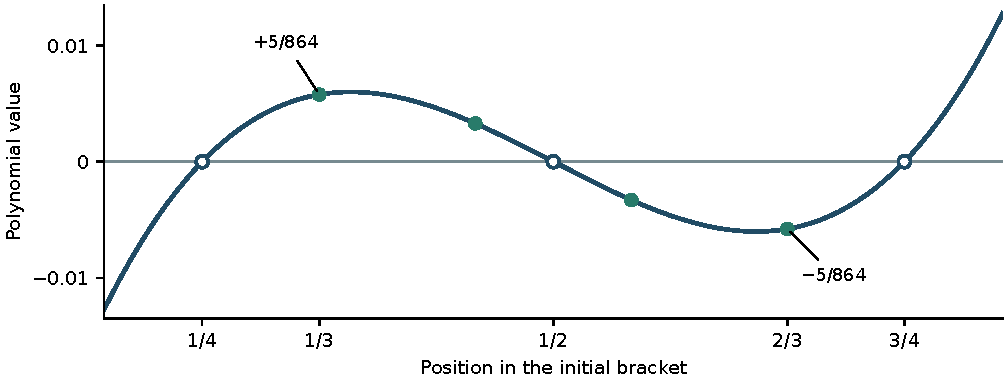
\includegraphics[width=.8\linewidth]{figures/root-probes.pdf}
\caption{Four middle-third probes of the cubic with roots at $1/4$, $1/2$ and $3/4$. The outer probes tie for largest magnitude, with opposite signs. Tiny admissible perturbations of the coefficient observations can break the tie in either direction.}
\end{figure}

\paragraph{Lean boundary.}
In \texttt{Root.lean}, \texttt{best} is the first maximizing index,
\texttt{difference\_bound} proves the $2^d$ estimate for successive
differences, and \texttt{monic\_peak} proves (R1) for an arbitrary
rational monic polynomial, degree, origin, and positive rational step.
It applies mathlib's factorial identity to $Q(u+hX)$ and uses that
polynomial's computed leading coefficient $h^d$. The lemma
\texttt{positive\_endpoint} is the sign-transport inequality for a
fixed target precision. These are checked ambient Lean theorems.
For the object-language endpoint encode the state as a rational endpoint
pair and let the PR step build a coefficient table, evaluate by Horner,
scan for the first maximum, and choose the subinterval by rational sign.
Use (R1)'s finite row proof above for the compiled difference-table
lemma, and (R2)'s two rational inequalities as the endpoint invariant.
Instantiate it twice for the desired endpoint precision and the final
sample comparison. Induct separately on a finite extension length for
nesting. These latter proof objects and the deep polynomial table
derivation remain to be constructed. The existing object proofs
\texttt{PolynomialBisection} and \texttt{PolynomialRootName} provide
the signed-rational bracket and regularity patterns at the pinned
revision.

\section{An entropy bound for compact families of functions}\label{sec:entropy}

A function space can itself be a domain for optimization. An important cost is the number of candidates in a finite net. For the bounded Lipschitz functions on a cube, ProveIt's second continuous-framework report assigns an independently quantized value to each grid vertex. It converts each table into a genuine Lipschitz function by taking a clipped minimum of cones. Its catalog has $B^S$ entries for $S$ vertices and $B$ possible values per vertex.\footnote{See \href{https://github.com/VladimirReshetnikov/ProveIt/blob/b2341af5370cd8a43f72ebb2341c0d7d7395b634/Logic/PrimitiveRecursiveArithmetic/docs/proofs/foundations/ipra_continuous_framework_2026-11-20_2/paper/sections/03_function_spaces.tex}{ProveIt, \emph{Compact presentations of spaces of functions}}, especially its envelope and net-size estimates.}
On the same spatial and value meshes, two extra bits per sample reduce the catalog to $B3^{S-1}$ entries. The construction below gives an address for a nearby function using one noisy evaluation at each grid vertex. The asymptotic order of metric entropy is classical. The result here is a numerically specified coding and decoding proof suitable for this iPRA presentation.\footnote{For the classical context see A.~N.~Kolmogorov and V.~M.~Tikhomirov, \href{https://www.mathnet.ru/eng/rm7289}{\emph{\(\varepsilon\)-entropy and \(\varepsilon\)-capacity of sets in function spaces}}, Uspekhi Mat. Nauk 14 (1959), 3--86.}

\subsection{One ternary digit per grid edge}

Use the maximum metric on $K=[0,1]^d$, $d\ge1$. Write $\mathcal F$ for the functions $K\to[-M,M]$ with Lipschitz constant at most the rational $L\ge0$, where $M\ge1$ is an integer and $s\ge0$ satisfies $L\le2^s$. The following symbols are local to this section. At requested error $e=2^{-k}$ put
\[
 \delta=e/4,\qquad m=k+3+s,\qquad h=2^{-m},\qquad
 S=(2^m+1)^d,\qquad B=2M/\delta+1.
\]
Hence $Lh\le\delta/2$. Enumerate all $S$ mesh vertices along one path with consecutive vertices at distance $h$. To construct the path in dimension zero use the single empty tuple. In dimension $j+1$, visit the layers of the first coordinate in increasing order. In even-numbered layers append the path of dimension $j$ forwards, and in odd-numbered layers append it backwards. Every vertex occurs exactly once. At a layer boundary the lower-dimensional coordinates match, so the step changes a single coordinate by $h$. These identities follow successively for the dimensions using bounded arrays of grid indices.

An address contains an integer $a_0$ with $-M/\delta\le a_0\le M/\delta$, followed by $S-1$ steps in $\{-1,0,1\}$. Decode by cumulative addition, giving integer labels $a_i$ at the successive vertices $v_i$. For every address let
\[
 P(x)=\operatorname{clip}_{[-M,M]}\min_{i<S}
           \{\delta a_i+L\|x-v_i\|_\infty\}.
\]
Here $\operatorname{clip}_{[u,v]}(t)=\max(u,\min(v,t))$. Every center is legal. The triangle inequality bounds the change of each cone by $L\|x-y\|_\infty$, hence bounds the change of their finite minimum by the same amount. Clipping is nonexpansive and forces the required range. This covers all addresses, including those for which a cumulative label leaves the original range. Values of centers at rational arguments are exact rationals.

\paragraph{Covering estimate.}
For a supplied $f\in\mathcal F$, query its value at every $v_i$ within $\eta=\delta/8$. Clip each answer into $[-M,M]$ to obtain a rational $u_i$, and put $a_i=\lfloor u_i/\delta+1/2\rfloor$. The endpoints are multiples of $\delta$, so $a_0$ is a legal first label. Consecutive clipped samples differ by at most $Lh+2\eta\le3\delta/4$. Rounding each adds at most $\delta/2$. Consequently $|a_{i+1}-a_i|\le7/4$. Integrality makes each difference an allowed step. The decoded table is exactly the rounded table.

At every vertex $|\delta a_i-f(v_i)|\le5\delta/8$. Each cone is at least $f(x)-5\delta/8$. For the other direction, a vertex within $h$ of $x$ gives a cone value at most $f(x)+5\delta/8+2Lh$. For rational $x$ use nearest mesh coordinates. For a named $x$, clip an approximation of error $h/4$ into the cube and round each coordinate to the nearest mesh value. The resulting distance is at most $3h/4$. Since clipping fixes $f(x)$, this proves
\[
 \|P-f\|_\infty\le 5\delta/8+2Lh\le13\delta/8=13e/32.
\]
The supremum notation abbreviates a uniform bound at every argument.

\paragraph{Cost and arithmetic meaning.}
Pack the root as an offset in $\{0,\ldots,B-1\}$ and the steps as a base-three word of length $S-1$. This gives $C=B3^{S-1}$ possible addresses. Center selection uses $S$ sample queries and $S-1$ local difference encodings. The saving concerns address size and exhaustive enumeration. For $d=M=L=1$, $s=0$, and $k=4$, the two catalogs on the same $129$ grid vertices require respectively $905$ and $210$ bits for a fixed-length address. Both counts are for addresses and can include duplicate functions. At the original sample precision $p=k+3$, errors up to $\delta/2$ give neighboring rounded labels differing by at most $5/2$ in mesh units, hence by at most two. Five possible increments then give $B5^{S-1}$ addresses and uniform error at most $\delta+2Lh\le e/2$, with the original sample budget. Even the smaller catalogs are expensive to enumerate.

For the numerical translation take a fixed PR evaluator $U(v,p)$ with
$|U(v,p)|\le M+2^{-p}$ and
$|U(v,p)-U(w,q)|\le L\|v-w\|_\infty+2^{-p}+2^{-q}$ at rational arguments. Then $p=k+5$ gives the stipulated sample error. These comparisons after multiplication by positive denominators are its arithmetic hypotheses. Clip the evaluator on both sides of its mixed Lipschitz bound. Nonexpansiveness preserves the bound, and the range hypothesis bounds the clipping change by $2^{-p}$, so this gives the same function name. For any rational $x$ the clipped sample at precision $q$ now plays the role of $f(x)$ in the cone proof with one additional $2^{-q}$ in the error. The finite proof takes the minimum over all the lower bounds and uses the grid witness for the upper bound. Its scan invariant says that the running minimum exceeds the common lower bound (weakly) and is at most every previously inspected cone. A bounded Boolean conjunction encodes the latter comparison. All clipping, rounding and digit operations are finite integer calculations. Even for variable $d$, the reflected path can be generated by dividing a rank into a layer and its remainder and reversing that remainder in odd layers, with at most $d$ divisions and reflections per vertex.

\subsection{How many bits are necessary?}

Take $M=L=1$, $k\ge3$, and put $J=2^{k-3}$. Form the $T=J^d$ grid sites $c$ whose coordinates belong to $\{0,8e,\ldots,8e(J-1)\}$. For each $T$-bit mask $b$ let
\[
 F_b(x)=\max\bigl(\{0\}\cup
       \{3e-\|x-c_i\|_\infty: i<T,\ b_i=1\}\bigr).
\]
Every $F_b$ is 1-Lipschitz, lies in $[0,1]$, and has an exact PR evaluator at rational points. At site $c_i$ its value is precisely $3e\,b_i$. Therefore any two distinct masks differ by at least $3e$ in supremum distance.

Every radius-$e$ net needs at least $2^T$ centers. This counting argument has a finite constructive form. For each supplied center sample its values at the $T$ sites within $e/4$, and decode a bit by comparing the sample to $3e/2$. If the center is within $e$ of $F_b$, the sample is at most $5e/4$ at an unmarked site and at least $7e/4$ at a marked site. Its decoded mask is exactly $b$. Coverage forces the list of decoded masks to include every $T$-bit word. Finite counting now gives the lower bound. For each fixed dimension, the lower and upper bounds on the base-two logarithm of the catalog size are both of order $2^{dk}$ as $k$ grows. Constants depend on $d$. An independent value at every vertex costs an additional factor of order $k$ in its logarithm.

\paragraph{Finite Arzelà--Ascoli consequence.}
Given $C(r-1)+1$ uniformly presented members of $\mathcal F$, $r\ge2$, assign each its address by the procedure above. A bounded count finds an address occurring at least $r$ times, since otherwise the total count is at most $C(r-1)$. Return the first $r$ associated indices. Their functions have pairwise distance at most $13e/16$. This provides a PR finite cluster operation for variable $r,k$ with a fixed family evaluator. The indices need not occur consecutively. A uniform selector of a convergent subsequence together with its regular limit name encounters an obstruction already for constant functions with values in $\{0,1\}$. On an all-zero sequence, a finite-use calculation of a $1/4$-approximation to the limit at the origin sees finitely many indices. Set all later entries to one. The calculation returns the same answer, yet every strictly increasing subsequence now has limit one. For an index-uniform computable selector the same obstruction follows by using the uniformly PR sequence of flags for a machine having halted within $n$ steps. Its limit within $1/4$ decides halting. The finite cluster result does not need consistency of selections across scales.

\paragraph{Lean realization.}
The file \texttt{Entropy.lean} proves the integer edge bound by writing the two clipped samples in units of $\delta$ as $X/D,Y/D$ with a common positive denominator. If $2Da\le2X+D$, $4X\le4Y+3D$, and $2Y\le2Db+D$, then $a\le b+1$. Otherwise $a\ge b+2$ contradicts the displayed inequalities. Interchanging the two vertices gives the other side. The nearest-integer implementation computes the signed Euclidean quotient $(2X+D)\mathbin{\mathrm{div}}(2D)$, and \texttt{roundNearest\_bounds} proves its error inequalities directly from the division law. The file proves that ternary decoding recovers the entire admissible tail of labels, that its encoding has one step per tail element, and that the exhaustive suffix catalog has length $3^n$ and contains every word of length $n$. For an object-language replay, define the reflected rank map and the address primitives as PR symbols. Prove the path properties by bounded checks on rank, dimension and coordinates. The envelope inequality then uses the minimum-scan invariant above. For the lower bound build the decoded mask for each address by a bounded scan and apply finite pigeonhole to the resulting mask table under the coverage premise. All induction predicates can use bounded Boolean and integer operations. The analytic interpretation is the dense-point extension of the Lipschitz inequalities.

\section{Formalization and reproducibility}
\label{sec:formal}
\subsection{What Lean checks}
The generator in \texttt{object/ObjectReplay.lean} imports the ordinary \texttt{ConciseIPRA.PR} judgment from ProveIt. A fixed finite tree has leaves that are object terms. Each address is assigned a term for its observed bit. A test with branches $l,r$ compiles to a ternary PR symbol $S(b,l,r)$ by primitive recursion on $b$, with base the first branch projection and successor case the second branch projection. The defining equations give $S(0,l,r)=l$ and $S(t+1,l,r)=r$. If $\Gamma$ proves the selected bit at each tested address on the path, structural induction on the tree yields an object derivation
\[
           \Gamma\vdash_{\rm PRAAx}
           \operatorname{compile}(\mathit{read},t)=\operatorname{selected}(\alpha,t).
\]
At a node substitute the proved bit by congruence, apply the appropriate defining equation, and compose with the subproof for that branch. No assumption is needed at an unvisited address. The theorem \texttt{replayTwo} applies this twice with different read routines. \texttt{exampleClosed} gives an unconditional closed object sentence. Both were replayed against the pinned repository sources. Lean reports only \texttt{propext} and \texttt{Quot.sound} in their metatheoretic axiom audit. The tree argument is external. A single object sentence quantifying over numerically coded trees is a further theorem.

\begin{center}\small
\begin{tabularx}{\linewidth}{@{}>{\raggedright\arraybackslash}p{.32\linewidth}X@{}}
\toprule Host Lean module & Checked statement\\ \midrule
\texttt{Dialogue} & Evaluation, replay from visited addresses, query substitution with exact trace, and a depth bound for substitution.\\
\texttt{Prefix}, \texttt{LeastPrefix}, \texttt{Oscillation} & Sparse compatibility characterizes extensions agreeing below $N$. On the actual pruned rows, the algorithm computes the least threshold controlling integer-output oscillation on all pairs of streams. A common denominator for labels and tolerance reduces Theorem~\ref{thm:least} to this result.\\
\texttt{Carry} & A representative in the finite list for the carry position preserves all comparisons against stored addresses. The finite existential test is equivalent to the unrestricted index test.\\
\texttt{CellGeometry}, \texttt{IntervalLift} & Clamped floor indices are equal or adjacent at one mesh width. Within-cell and boundary estimates give (1). From (1) and same-input coherence the explicit lift satisfies mixed regularity, extensionality and the Euclidean modulus bound.\\
\texttt{BitIntegral}, \texttt{FiniteCube}, \texttt{DepthMean} & Finite-cube partition, mass splitting at fresh bits and reuse of a forced bit. The depth-$D$ numerator with denominator $2^D$ equals the full cube average after cross multiplication.\\
\texttt{Root} & Finite-difference peak bound for a rational monic polynomial with an actual maximizing index, and transport of a positive certified sign to a later weak endpoint inequality.\\
\texttt{Entropy} & Integer rounding, extraction and decoding of ternary edge differences, and completeness and length of the enumeration of words.\\
\bottomrule
\end{tabularx}
\end{center}
The standard-library modules and the Mathlib proofs were replayed with Lean 4.32.0. The executable checks compared the sparse algorithm with complete truth tables on 140 generated trees, including repeated queries, and compared 80 mixed Cauchy-name samples. Additional exact-rational checks cover the metric triangle, weak intermediate values, polynomial brackets, roundoff on Lipschitz edges, envelopes and packing masks. The verification folder gives commands and results. These finite checks exercise the implementations. The remaining host-level link identifies the prefixes of the rational binary-digit routine and the carry expansions with the geometric cell and boundary labels. That link has a human proof, as do the Riemann adequacy theorem, full polynomial-bracket algorithm and entropy bounds. The following steps specify how to obtain the remaining deep object-language proofs.

\subsection{A route to the object sequents}
\paragraph{1. Code the data.}
One standalone encoding takes $\operatorname{nil}=0$ and $\operatorname{cons}(a,t)=2^a(2t+1)$. The head of a nonzero code is the exponent of two dividing it, bounded by the code. The tail is the remaining odd part minus one, divided by two. The tail is strictly smaller. Length, indexing, lookup, membership, reverse and append are therefore PR by bounded iteration. Pairs use the same positive encoding. Encode a signed integer by sign and magnitude, a rational by a signed numerator and positive denominator, and a row by a list of distinct address/bit pairs and a rational label. Set total defaults on bad input. Comparisons use cross products with a positive-denominator guard. Normalization of rational fractions is optional.

A port can use the repository's \repo{Derivations/Lean/IPRADerivations/Foundations/DigitCodes.lean}{digit code lemmas}, \repo{Derivations/Lean/IPRADerivations/Foundations/DyadicNames.lean}{dyadic bounds}, and \repo{Derivations/Lean/IPRADerivations/Analysis/RationalArithmetic.lean}{rational arithmetic}. Check the scope of each imported result. Some digit lengths in \texttt{DigitCodes} are external naturals. Variable-length loops here need numerical folds and proofs of their defining equations.

\paragraph{2. Produce the rows.}
Fix the machine step term. Define the padded $B$-bit simulation of Section~\ref{sec:framework}, with state consisting of machine state, remaining fuel, a fresh-answer cursor and partial map. At an old address use the lookup without advancing the cursor. At a new address read the cursor bit, extend the map and advance. Scan all words below $2^B$, emitting each distinct terminal transcript once by bounded comparison. For a frozen input word the loop invariant states that all recorded answers agree with this input and that replay of the trace prefix reaches the stored state. Its bounded version tests each recorded index through the current step. With a second input that agrees on the stored addresses, either simulation makes the same next transition. To prove coverage, record the fresh replies of a given finite input in order and pad with zeros. For the converse replay with the finite-support extension. Freeze two distinct rows and find the first unequal fresh reply to prove disjointness. Check the halt test also in the state reached at time $B$. These constructions provide the uniform counterpart of the fixed-tree result. The repository's \repo{Derivations/Lean/IPRADerivations/Foundations/TraceComposition.lean}{trace-composition proof} illustrates freezing auxiliary parameters.

\paragraph{3. Prove compatibility and one-cell geometry.}
Use a first-element initializer and a left fold for minimum on a nonempty list. The invariant says the stored extremum bounds all processed values and belongs to the processed list. Compile the universal part into a bounded Boolean conjunction. Compare each forbidden pair with its least shared conflicting address. The counterexample extensions are the explicit PR functions of Theorem~\ref{thm:least}. For (G), replace an index $j$ absent from the keys by the maximum of zero and the successors of keys below it. No stored bit changes position relative to $j$. On the mesh $2^{-N}$, the one-cell estimate reduces to
\[
 x\le y\le x+2^{-N}\quad\Longrightarrow\quad
        \lfloor2^Ny\rfloor\le \lfloor2^Nx\rfloor+1 .
\]
Prove this by division with remainder, then clamp both indices at $2^N-1$. Neighboring indices have binary forms $u0\,11\cdots1$ and $u1\,00\cdots0$ of length $N$. Use bounded search for the last zero in the smaller word. Adding one changes precisely this suffix. This covers both end cells. With (C) and (G) this gives (1) as a sequent about rational point codes.

\paragraph{4. Close the indices of the analytic contracts.}
For the actual term $y(a,n)$ in Theorem~\ref{thm:interval}, one endpoint is the universal closure, under the tests (C), (G) and the input guards, of
\[
 \operatorname{EqName}(a,b)\ \longrightarrow\
 |y(a,n)-y(b,m)|\le 2^{-n}+2^{-m}.
\]
Here $a,b$ abbreviate fixed PR sample terms with numerical parameters, and $\operatorname{EqName}$ is the mixed cross-index inequality of Section~\ref{sec:framework}. Construct the envelope $H$ by a bounded max, then instantiate the one-cell theorem on the two computed sample codes. For the modulus endpoint use the mixed inequality with input distance $\le2^{-\mu(j)}$ and output distance $\le2^{-j}$, including both sample errors. A fully finite proof freezes output indices $i,l$ and compares both outputs through two level-$s$ samples at $s=\max(i,l,j+2)$. Their inputs are within the one-cell threshold at level $j+2$. Using (C) to compare the two fine outputs through that level costs at most $\eps_j+2\eps_{s+3}$. Transporting the original outputs to the two fine ones costs at most $3\eps_{i+3}+\eps_{s+3}$ and $3\eps_{l+3}+\eps_{s+3}$. Since $\eps_s\le\min(\eps_i,\eps_l)$, the total fits $\eps_i+\eps_j+\eps_l$. This is the proof implemented in \texttt{IntervalLift}. All indices are numerical inputs, with no induction on convergence formulas.

For integration, track the remaining free coordinates during finite cube enumeration. At an unfixed query, flipping exactly that bit matches the two subpopulations bijectively. At a fixed query the full population follows the known branch. Sum scaled integer values and prove the cross-product identity before dividing by positive denominators. In the tagged-partition proof merge the sorted lists of endpoints. The invariant preserves covered length and the accumulated error bound. For the polynomial and entropy endpoints, Sections~\ref{sec:root-realizer} and \ref{sec:entropy} give the specific numerical invariants. Each final target is a sequent $\Gamma\vdash_{\rm PRAAx}\varphi$ for the chosen PR providers. The \repo{Bridge/README.md}{Foundation--Concise bridge} can transport such a proof to the other arithmetic presentation.

\paragraph{5. Interpret the result.}
A regular output with the mixed inequalities denotes a point of the completion. An integral name agreeing with sufficiently fine Riemann sums denotes the Riemann integral. For a multivalued operation the endpoint asserts that each output satisfies its defining relation. Requiring all legal coefficient names to select the same root would strengthen that statement, as the cubic example shows.

\subsection{Further research questions}
\begin{enumerate}[leftmargin=22pt]
\item Can shared subtrees across precisions shorten independently checkable certificates for the least oscillation threshold and for the integral? A benchmark would compare certificate sizes on functions with many repeated queries.
\item For power-series or piecewise analytic inputs, which coefficient bounds can replace $d!h^d$? The bracket theorem needs just one robust sign in every middle third. Producing such a bound from natural analytic data would extend the root theorem.
\item On compact metric spaces presented by nets with bounded branching, when do a ternary edge code and a bump packing give matching entropy bounds? The cube proof identifies the need for both a short traversal and a large separated family.
\end{enumerate}

\begin{thebibliography}{9}
\bibitem{repo} V. Reshetnikov and contributors, \emph{ProveIt, Primitive Recursive Arithmetic}. \repo{README.md}{Pinned source overview}, revision \texttt{b2341af5370cd8a43f72ebb2341c0d7d7395b634}. Individual modules and packet comparisons are linked where used.
\bibitem{escardo} M. Escard\'o, \emph{Continuity of G\"odel's System T definable functionals via effectful forcing}, Electronic Notes in Theoretical Computer Science 298 (2013), 119--141. \href{https://doi.org/10.1016/j.entcs.2013.09.010}{Article and DOI}.
\bibitem{pauly} A. Pauly, \emph{On the topological aspects of the theory of represented spaces}, Computability 5 (2016), 159--180. \href{https://arxiv.org/abs/1204.3763}{Author's paper}.
\bibitem{oconnor} R. O'Connor, \emph{A monadic, functional implementation of real numbers}, Mathematical Structures in Computer Science 17 (2007), 129--159. \href{https://arxiv.org/abs/cs/0605058}{Author's paper}. See also the completion and lifting construction there.
\end{thebibliography}

\end{document}
